% Options for packages loaded elsewhere
\PassOptionsToPackage{unicode}{hyperref}
\PassOptionsToPackage{hyphens}{url}
%
\documentclass[
]{article}
\usepackage{amsmath,amssymb}
\usepackage{iftex}
\ifPDFTeX
  \usepackage[T1]{fontenc}
  \usepackage[utf8]{inputenc}
  \usepackage{textcomp} % provide euro and other symbols
\else % if luatex or xetex
  \usepackage{unicode-math} % this also loads fontspec
  \defaultfontfeatures{Scale=MatchLowercase}
  \defaultfontfeatures[\rmfamily]{Ligatures=TeX,Scale=1}
\fi
\usepackage{lmodern}
\ifPDFTeX\else
  % xetex/luatex font selection
\fi
% Use upquote if available, for straight quotes in verbatim environments
\IfFileExists{upquote.sty}{\usepackage{upquote}}{}
\IfFileExists{microtype.sty}{% use microtype if available
  \usepackage[]{microtype}
  \UseMicrotypeSet[protrusion]{basicmath} % disable protrusion for tt fonts
}{}
\makeatletter
\@ifundefined{KOMAClassName}{% if non-KOMA class
  \IfFileExists{parskip.sty}{%
    \usepackage{parskip}
  }{% else
    \setlength{\parindent}{0pt}
    \setlength{\parskip}{6pt plus 2pt minus 1pt}}
}{% if KOMA class
  \KOMAoptions{parskip=half}}
\makeatother
\usepackage{xcolor}
\usepackage[margin=1in]{geometry}
\usepackage{graphicx}
\makeatletter
\def\maxwidth{\ifdim\Gin@nat@width>\linewidth\linewidth\else\Gin@nat@width\fi}
\def\maxheight{\ifdim\Gin@nat@height>\textheight\textheight\else\Gin@nat@height\fi}
\makeatother
% Scale images if necessary, so that they will not overflow the page
% margins by default, and it is still possible to overwrite the defaults
% using explicit options in \includegraphics[width, height, ...]{}
\setkeys{Gin}{width=\maxwidth,height=\maxheight,keepaspectratio}
% Set default figure placement to htbp
\makeatletter
\def\fps@figure{htbp}
\makeatother
\setlength{\emergencystretch}{3em} % prevent overfull lines
\providecommand{\tightlist}{%
  \setlength{\itemsep}{0pt}\setlength{\parskip}{0pt}}
\setcounter{secnumdepth}{-\maxdimen} % remove section numbering
\ifLuaTeX
  \usepackage{selnolig}  % disable illegal ligatures
\fi
\usepackage{bookmark}
\IfFileExists{xurl.sty}{\usepackage{xurl}}{} % add URL line breaks if available
\urlstyle{same}
\hypersetup{
  pdftitle={Análisis multivariado},
  hidelinks,
  pdfcreator={LaTeX via pandoc}}

\title{Análisis multivariado}
\author{}
\date{\vspace{-2.5em}}

\begin{document}
\maketitle

\begin{verbatim}
## [1] FALSE
\end{verbatim}

\begin{verbatim}
## [1] FALSE
\end{verbatim}

\begin{center}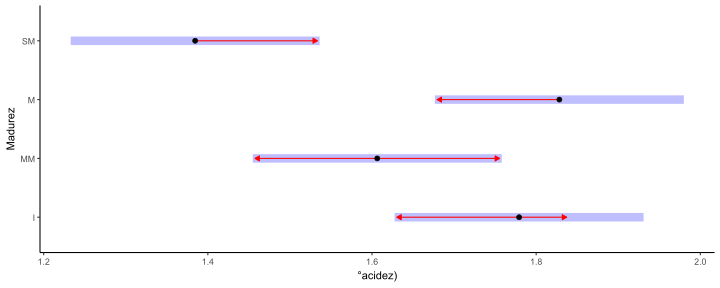
\includegraphics[width=0.95\linewidth]{V_Multivariate_files/figure-latex/unnamed-chunk-20-1} \end{center}

\begin{center}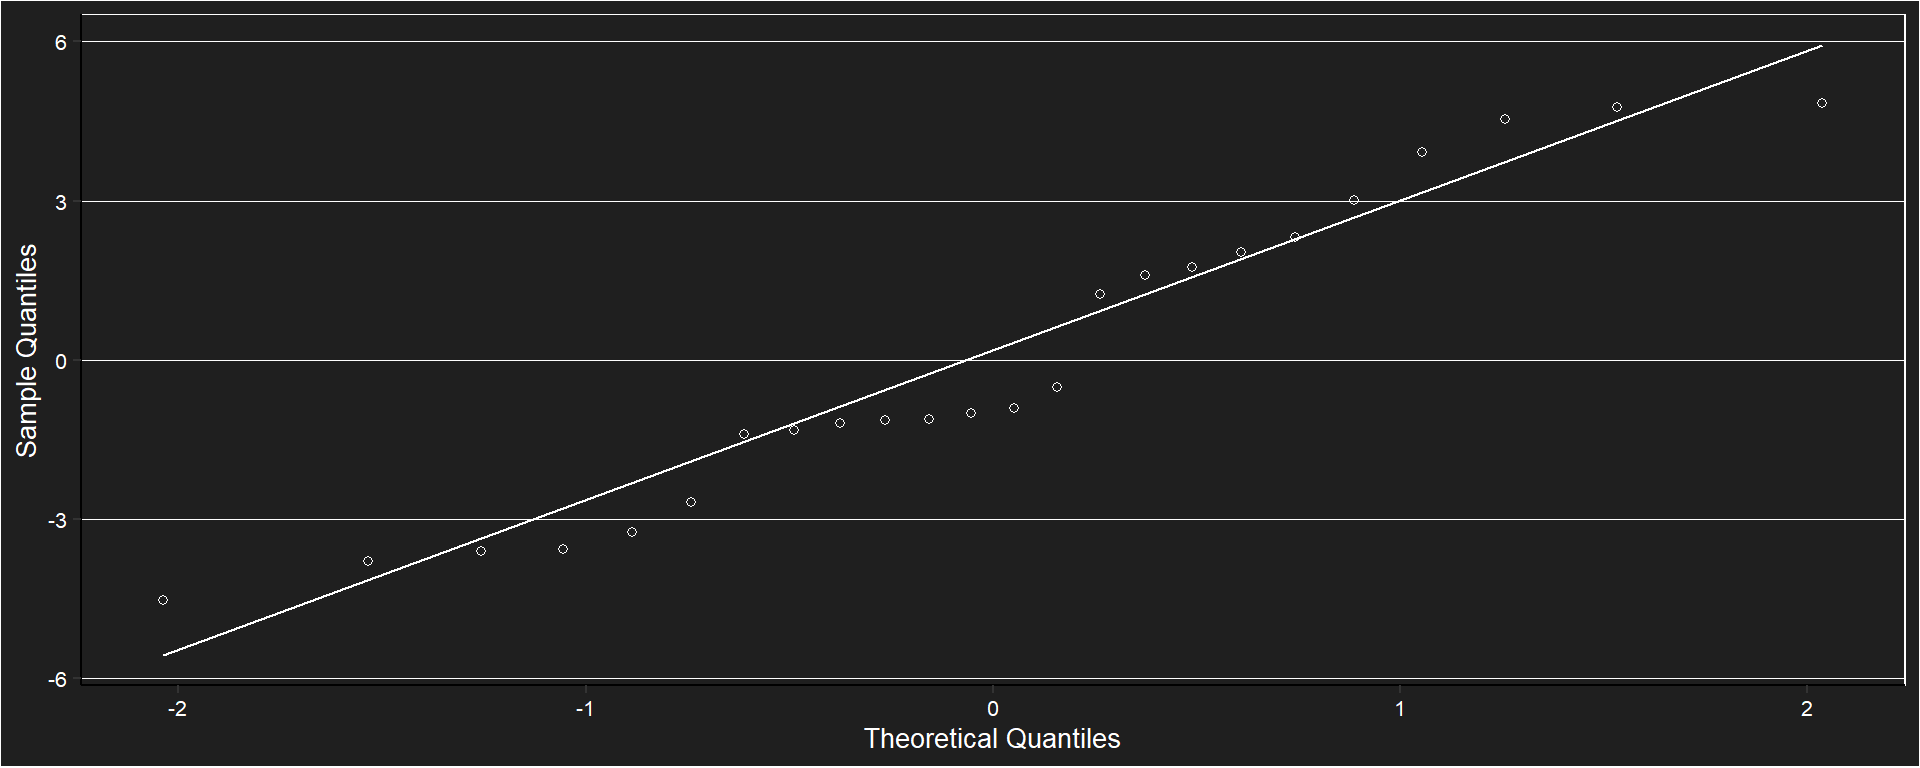
\includegraphics[width=0.95\linewidth]{V_Multivariate_files/figure-latex/unnamed-chunk-20-2} \end{center}

\begin{center}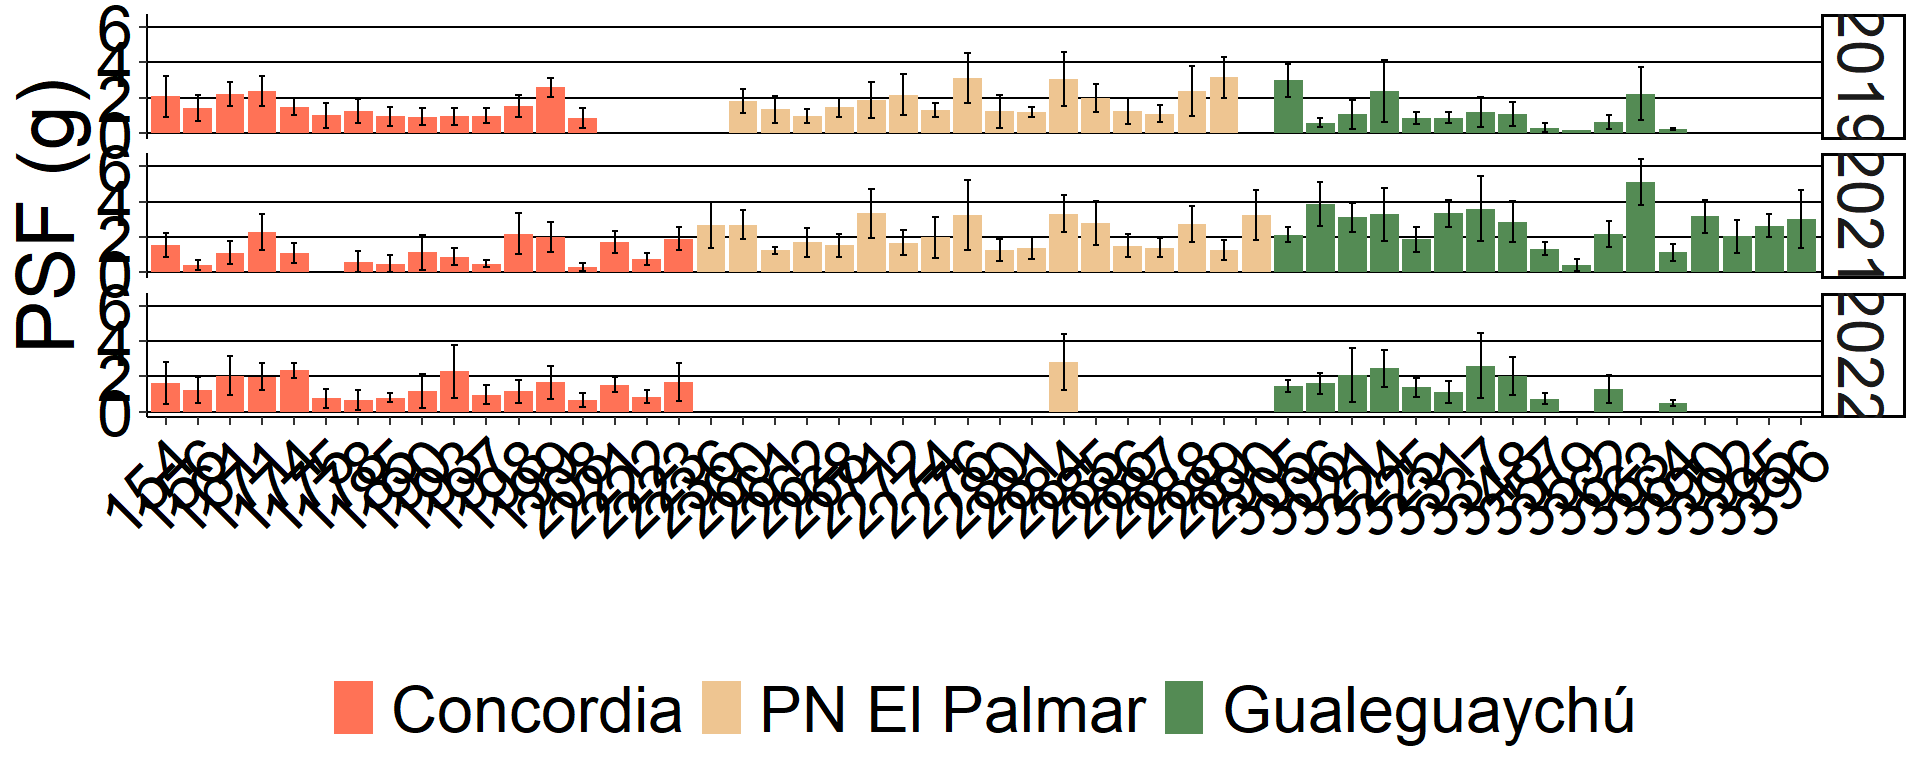
\includegraphics[width=0.95\linewidth]{V_Multivariate_files/figure-latex/unnamed-chunk-21-1} \end{center}

\begin{center}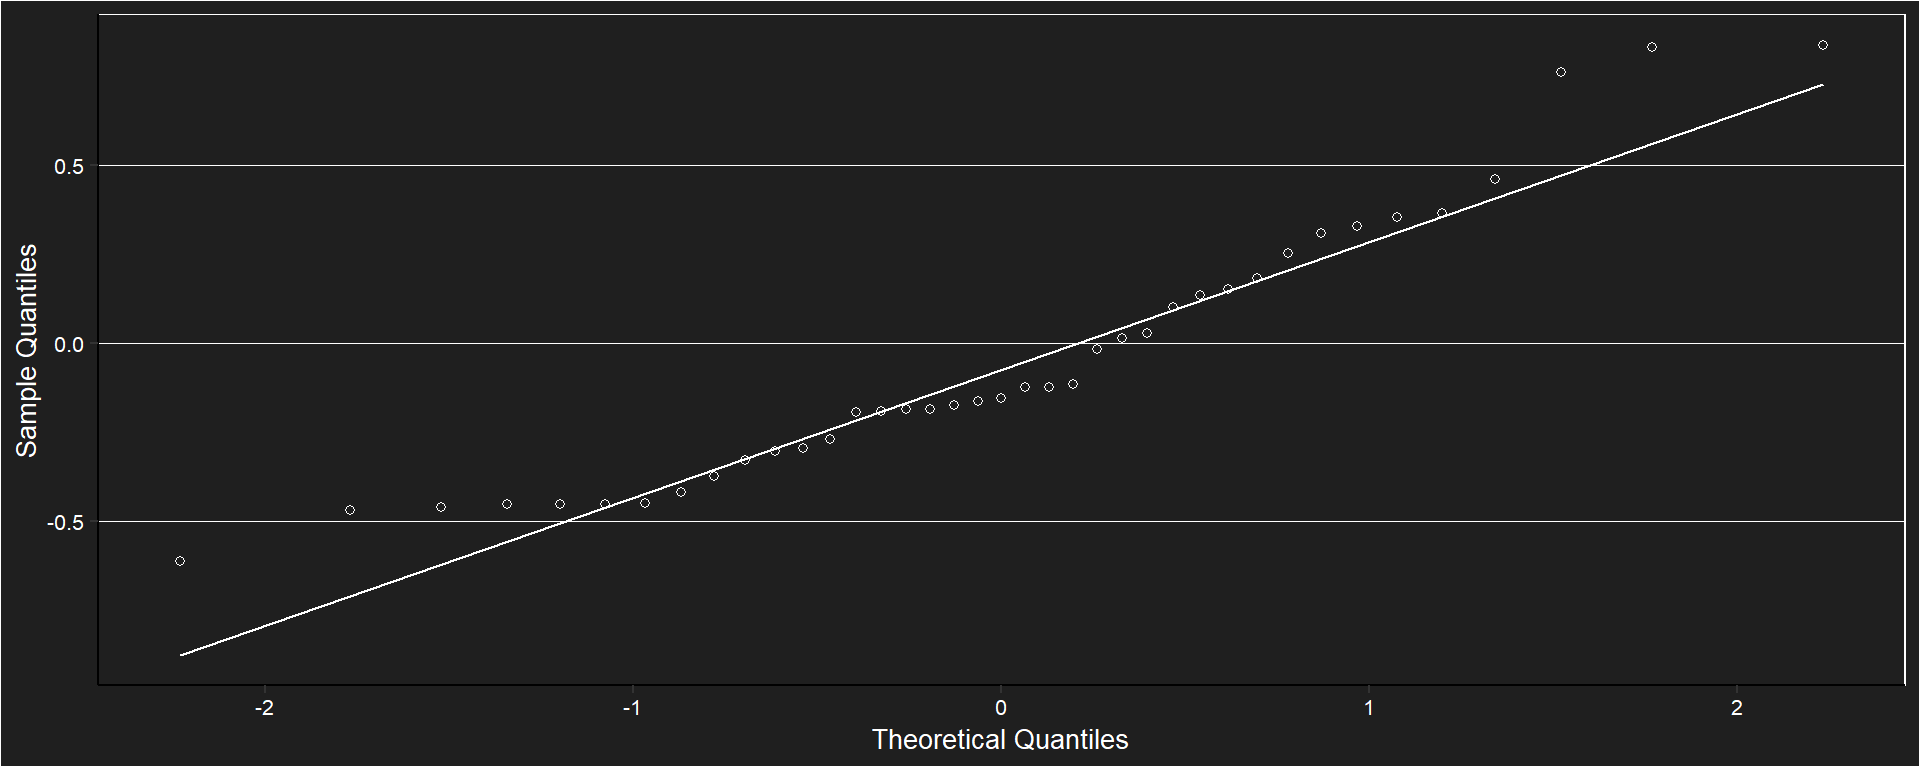
\includegraphics[width=0.95\linewidth]{V_Multivariate_files/figure-latex/unnamed-chunk-21-2} \end{center}

\begin{verbatim}
##        pen     indmad         de        phi        pff    color_a      ratio         ac        psf       clob       cloa        pss        fen         dp      aao25 
## 8.70827124 7.76789015 7.53413101 7.27058886 7.02575009 6.54985768 6.29330913 5.94357995 5.76768814 5.67273054 5.65990543 4.81306905 4.61070417 4.05428449 3.06975408 
##        ph8      aao50    color_b     aao100       caro       brix    color_L         ns     aao250 
## 2.63564975 2.18002277 1.29162007 1.25386278 1.14500902 0.51619777 0.18318633 0.03196175 0.02097578
\end{verbatim}

\begin{verbatim}
##    color_L    color_b         dp        pff        psf        pss         de       brix       cloa       clob         ns     aao100         ac     indmad      ratio 
## 12.7458133 11.0571486  8.6185104  7.0304350  6.8346191  6.3341881  5.5738117  3.5306837  3.5237796  3.5225865  3.2896165  3.2887871  2.9101485  2.6768755  2.6667901 
##     aao250        fen        phi    color_a      aao50      aao25        pen        ph8       caro 
##  2.6095983  2.5532503  2.1928534  2.0297828  1.9890855  1.9473648  1.5279107  1.4417688  0.1045918
\end{verbatim}

\subsection{Supresión de variables}\label{supresiuxf3n-de-variables}

\begin{verbatim}
##     pff      de color_L      dp     psf color_b     pss  indmad     pen     phi    clob    cloa   ratio      ac color_a     fen   aao25  aao100   aao50     ph8    brix 
##   14.06   13.10   12.93   12.67   12.60   12.35   11.14   10.45   10.24    9.46    9.19    9.18    8.96    8.85    8.58    7.16    5.02    4.54    4.17    4.08    4.05 
##      ns  aao250    caro 
##    3.32    2.63    1.25
\end{verbatim}

\begin{verbatim}
## [1] FALSE
\end{verbatim}

\begin{verbatim}
## [1] FALSE
\end{verbatim}

\begin{center}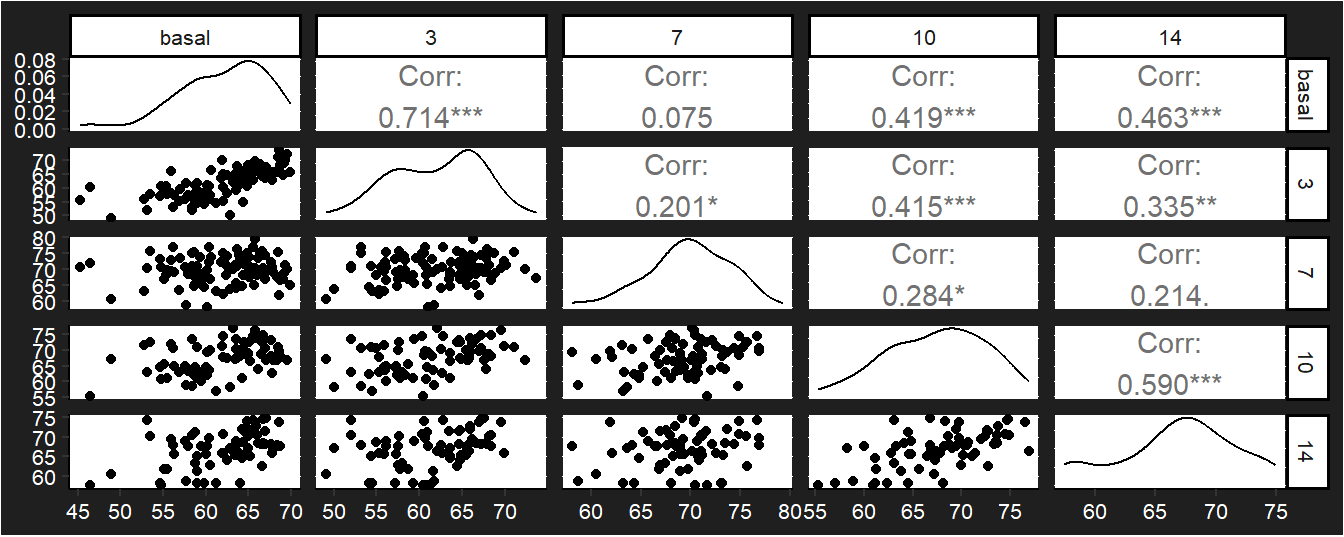
\includegraphics[width=0.95\linewidth]{V_Multivariate_files/figure-latex/unnamed-chunk-23-1} \end{center}

\begin{center}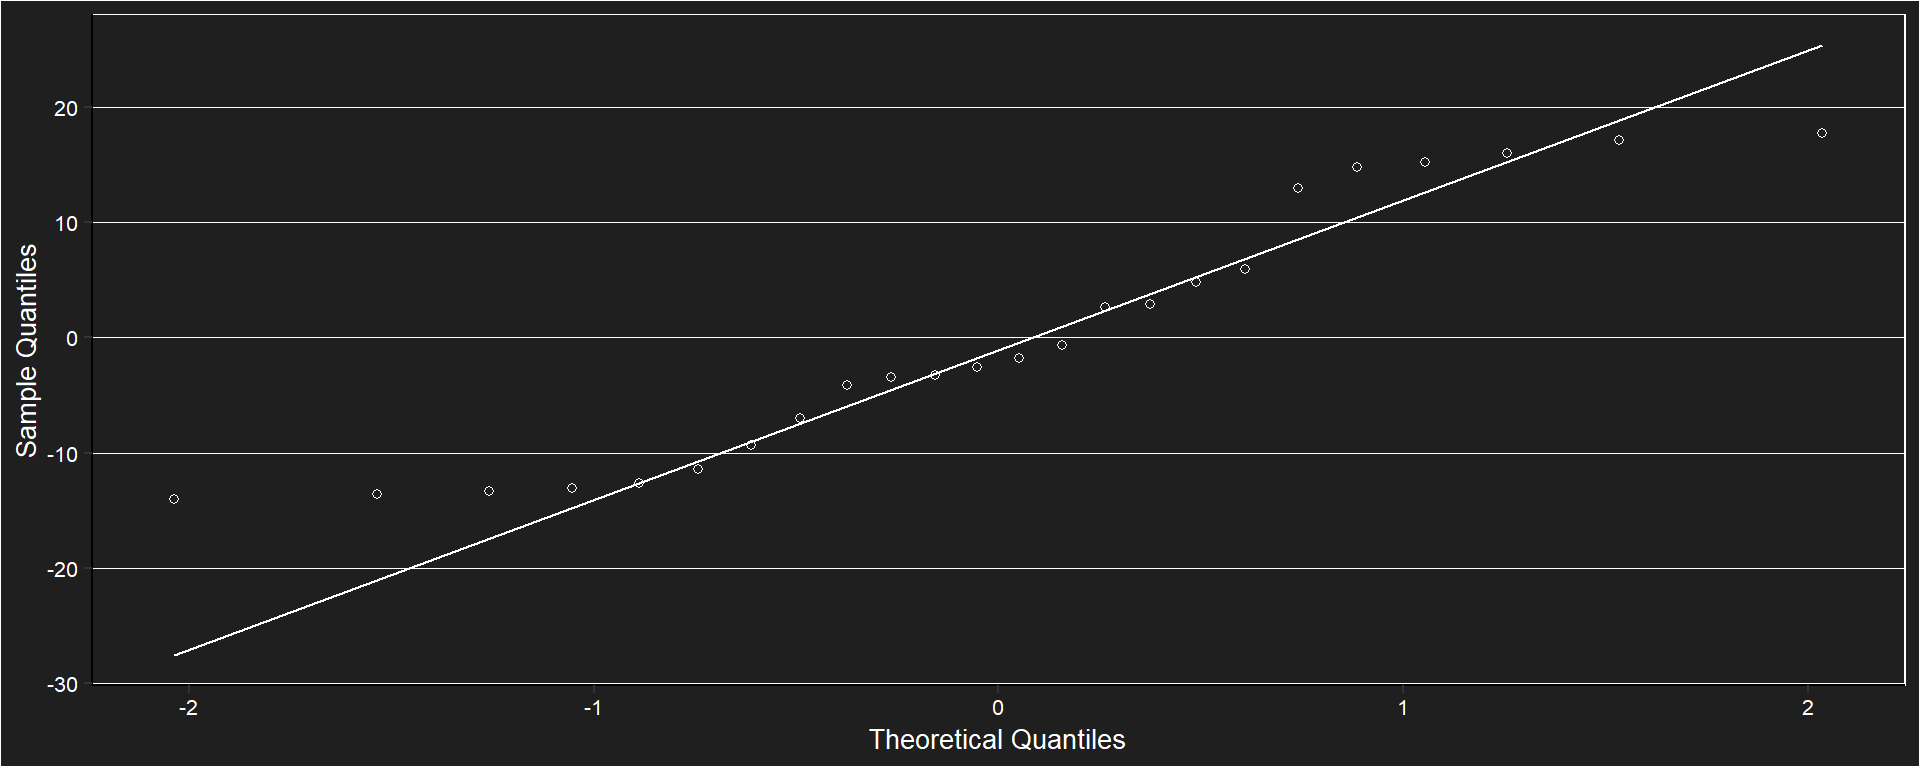
\includegraphics[width=0.95\linewidth]{V_Multivariate_files/figure-latex/unnamed-chunk-23-2} \end{center}

\begin{verbatim}
## Error in `geom_text_repel()`:
## ! Problem while computing aesthetics.
## i Error occurred in the 8th layer.
## Caused by error:
## ! objeto 'phenotype' no encontrado
\end{verbatim}

\begin{verbatim}
## Error in `geom_text_repel()`:
## ! Problem while computing aesthetics.
## i Error occurred in the 8th layer.
## Caused by error:
## ! objeto 'phenotype' no encontrado
\end{verbatim}

\begin{verbatim}
##       pen        de    indmad       phi       pff   color_a     ratio       psf        ac      clob      cloa       pss       fen        dp     aao25   color_b   color_L 
## 9.4979398 8.5296807 8.3292185 8.0039985 7.7488815 7.0460675 6.7995607 6.4859841 6.2437314 5.9496840 5.9348866 5.5016436 4.9218707 4.5658386 2.5588112 1.6171295 0.2650731
\end{verbatim}

\begin{verbatim}
##   color_L        dp   color_b       psf       pff       pss        de      cloa      clob    indmad     ratio       phi       pen        ac   color_a       fen     aao25 
## 13.861935 11.580254 11.336556 10.648967  9.504779  9.320923  7.367315  4.905522  4.903379  3.536766  3.132359  2.280262  2.116587  2.021715  1.670050  1.621173  0.191458
\end{verbatim}

\begin{center}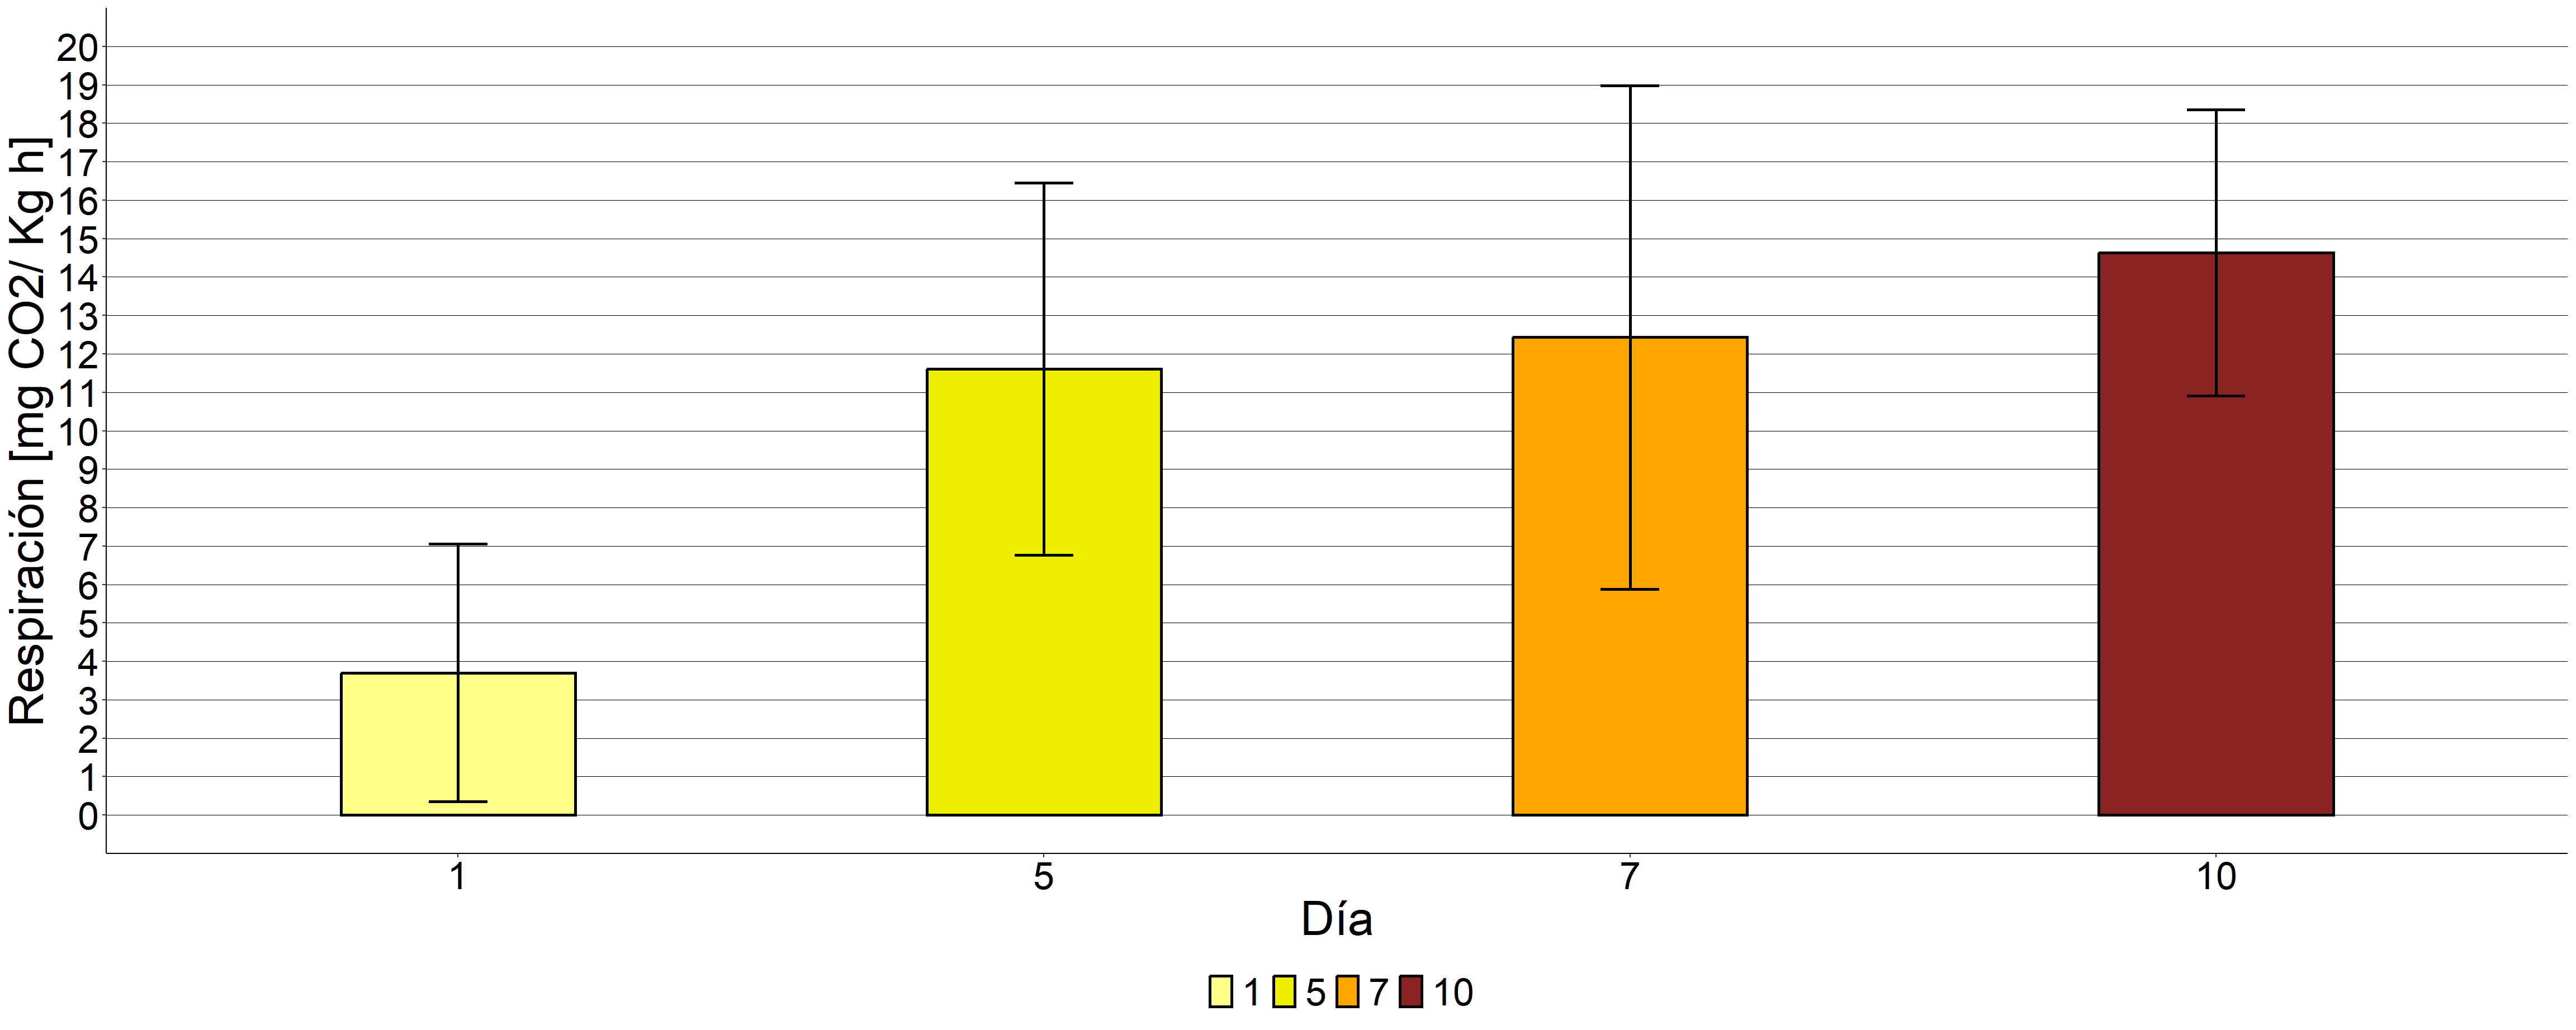
\includegraphics[width=0.95\linewidth]{V_Multivariate_files/figure-latex/unnamed-chunk-26-1} \end{center}

\section{Análisis univariado}\label{anuxe1lisis-univariado}

\begin{center}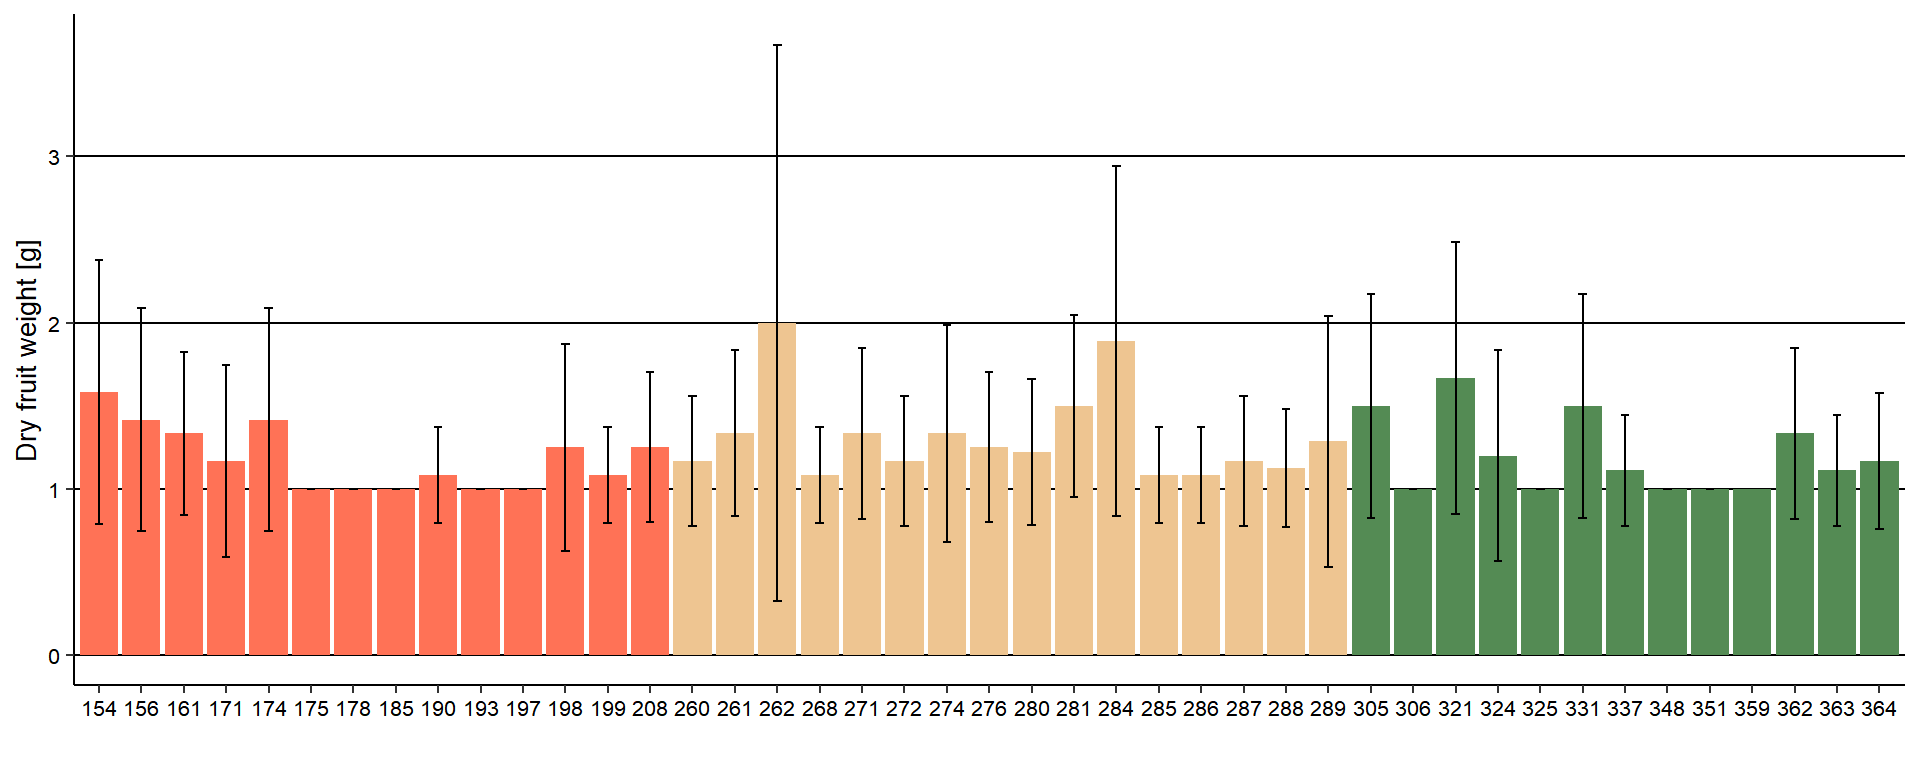
\includegraphics[width=0.95\linewidth]{V_Multivariate_files/figure-latex/unnamed-chunk-28-1} \end{center}

\begin{itemize}
\item
  QUIM chemical variables
\item
  FIS physical variables
\item
  PFF Peso fresco del fruto
\item
  DE Diámetro ecuatorial
\item
  DP Diámetro polar
\item
  PEN Resistencia a la penetración
\item
  PSF Peso seco del fruto
\item
  PSS Peso seco semilla
\item
  IM Índice de madurez
\item
  AAO Actividad Anti Oxidante
\item
  CAR Carotenoides
\item
  CLOA Clorofila a
\item
  CLOB Clorofila b
\item
  PHE Fenoles totales
\item
  TSS Solidos solubles totales
\item
  TTA Acidez Total Titulable
\item
  POB population
\item
  IND phenotype
\item
  RES residual
\end{itemize}

\end{document}
